Meshroom je brezplačno odprtokodno orodje za 3D rekonstrukcijo, ki jo je razvilo podjetje AliceVision. Glavni način uporabe je povezovanje vozlišč, ki računajo podatke. Za začetek odprite Meshroom, izberite File$\rightarrow$New Pipeline$\rightarrow$Photogrammetry, povlecite in spustite slike predmeta, ki ga želite rekonstruirati, v galerijo slik in pritisnite Start. Ko vozlišča končajo z računanjem, jih lahko dvakrat kliknete, da si ogledate njihove rezultate. \cite{Meshroom}

\section{Vozlišča}

\subsection{CameraInit}
    To vozlišče obdela dane slike v podatke, ki jih Meshroom lahko uporabi. Prav tako bere metadata s slik, da pridobi informacije, ki jih je mogoče pozneje uporabiti v cevovodu, na primer goriščno razdaljo ali notranje parametre kamere.


\subsection{FeatureExtraction}
    To vozlišče iz slik izvleče različne točke, imenovane ``features". V njegovih parametrih lahko določimo, katero metodo lahko uporabimo. Privzeta in velikokrat najboljša metoda je dspsift (domain size pooling scale invariant feature transform), vendar obstaja tudi metoda akaze, ki se lahko uporablja za zahtevne površine, kot je koža. Tukaj lahko določimo tudi ekstrahiranje točk s cctags, ki jih lahko uporabimo za skaliranje končnega modela, tako da določimo položaje teh oznak v resničnem svetu (Opomba: če uporabljate cctags, mora imeti vsaka slika vsaj 1 viden cctag in slike je treba zmanjšati na približno 1920x1080, ker ima trdo kodirano omejitev MAX\_RESOLUTION).
    V nastavitvah tega vozlišča lahko podamo tudi maske za slike, tako da ekstrahira samo točke v danem polju na sliki. Prav tako lahko spremenimo količino in kakovost pridobljenih točk.
    
\subsection{ImageMatching}
    To vozlišče se ujema s slikami, tako da vemo, katere slike so blizu, da jih lahko pozneje uporabimo za FeatureMatching. Obstaja več metod ImageMatching. VocabularyTree razvršča in primerja ekstrahirane lastnosti vsake slike. Sequential ujema slike na podlagi njihovega imena. Exhaustive ujema vsako sliko z vsako sliko. Frustum ujema na podlagi znanih poz in ujema slike v bližini.

\subsection{FeatureMatching}
    To vozlišče pregleda najdene pare slik in najde podobne lastnosti na obeh slikah. V nastavitvah je parameter, imenovan minimal 2D motion. Privzeto je -1, kar pomeni onemogočeno, če pa ga postavimo na neko pozitivno vrednost, na primer 2, določimo, da se točka, ki naj se ujema, ne sme biti v istem položaju na obeh slikah. Ta možnost je uporabna za filtriranje ujemanj v ozadju, če uporabljamo vrtljive mize, ker je ozadje statično.

\subsection{StructureFromMotion}
    To vozlišče uporablja ta ujemanja in te podatke uporablja za prikaz položaja teh točk v 3D-prostoru ter poze (položaj in orientacija) in notranje kalibracije vseh kamer.

\subsection{PrepareDenseScene}
    To vozlišče nepopači slike. Za izračun nepopačenih slik uporablja kalibracijske parametre iz StructureFromMotion.

\subsection{DepthMap and DepthMapFilter}
    Ta vozlišča izračunajo globino slik. Filter izloči nekoherentne vrednosti globine. Določimo lahko faktor znižanje, nižji kot je faktor, večja je kakovost, a daljši je čas izračuna. 1 bi morali uporabiti samo, če imamo zelo kakovostne slike.

\subsection{Meshing and MeshFiltering}
    Mreže se izvajajo iz podatkov SfM in globin. Rezultat je gosta geometrijska površinska predstavitev scene. To mrežo lahko nato uporabimo laplaciansko filtriranje, da odstranimo lokalne napake. V nastavitvah lahko določimo vrsto izhodne datoteke, ki jo najdemo v mapi MeshroomCache, in jo lahko odpremo in manipuliramo z drugimi aplikacijami, kot je Blender.

\subsection{Texturing}
    To vozlišče teksturira mrežo. Za vsak trikotnik uporabi informacije o vidnosti, povezane z vsakim vozliščem, da pridobi kandidate za teksturo. Izbere najboljše kamere glede na ločljivost, ki pokriva trikotnik. Končno izračuna povprečje vrednosti slikovnih pik z uporabo več pasov v frekvenčni domeni.

\section{Post processing}
    Uporabimo lahko aplikacijo, kot je Blender, da si ogledamo in manipuliramo z mrežo rezultatov. Najpogosteje lahko izrežemo neželene dele iz naše mreže, skaliramo mrežo na podlagi znane geometrije in nato opravimo meritve rekonstruiranega objekta.

\section{Rezultati}
    Da bi prikazali funkcionalnost Meshrooma, bomo analizirali naslednje rekonstrukcije, ki sem jih naredil in jih naknadno obdelal v Blenderju.

    \subsection{Kitara}
    Ta model je bil narejen iz 310 slik iz različnih kotov. Kitara je bila postavljena na sredino mize, miza pa med 2 stropni svetilki, tako da je osvetlitev večinoma enaka z obeh strani. Slike so bile posnete s telefonom, ki sem ga držal. Ker sem ga držal in moja roka ni zelo stabilna, sem moral uporabiti nizka hitrost zaklopa, 1/25 s na teh slikah, zaradi česar so bile slike temne, in v nasprotju s tem sem uporabil visok ISO faktor 1200. Na mizo sem postavil tudi CCTags, vendar mi je Meshroom povzročal težave pri skaliranju, kar bom v prihodnosti popravil, in jih uporabil v Blenderju za skaliranje modela. Iz rezultatov lahko vidimo, da je bil velik del moje sobe rekonstruiran iz ozadja slik, čeprav ne preveč podrobno. Ena od stvari, ki jih Meshroom uporablja za ujemanje, so tudi podrobnosti ozadja, kar je v tem primeru super, ker je vsak kot ozadja edinstven. Kitaro sem izrezal iz modela v Blenderju. Vidimo lahko, da so vrat kitare in nesijajni deli zelo dobro rekonstruirani. Največja napaka je v trupu kitare. Tam, kjer je kitara najbolj sijoča, je velika luknja, to je zaradi odseva svetilk na trupu kitare. V prihodnosti se to lahko odstrani z uporabo polarizacijskega filtra, z mat barvo na predmetu ali z boljšo osvetlitvijo. Tudi slike za ta model so bile posnete v formatu JPG in RAW. Rezultati rekonstrukcije so pokazali, da so JPG slike veliko boljše od tistih v RAW formatu.
    
        \begin{figure}[h]
            \begin{subfigure}{.5\textwidth}
                \centering
                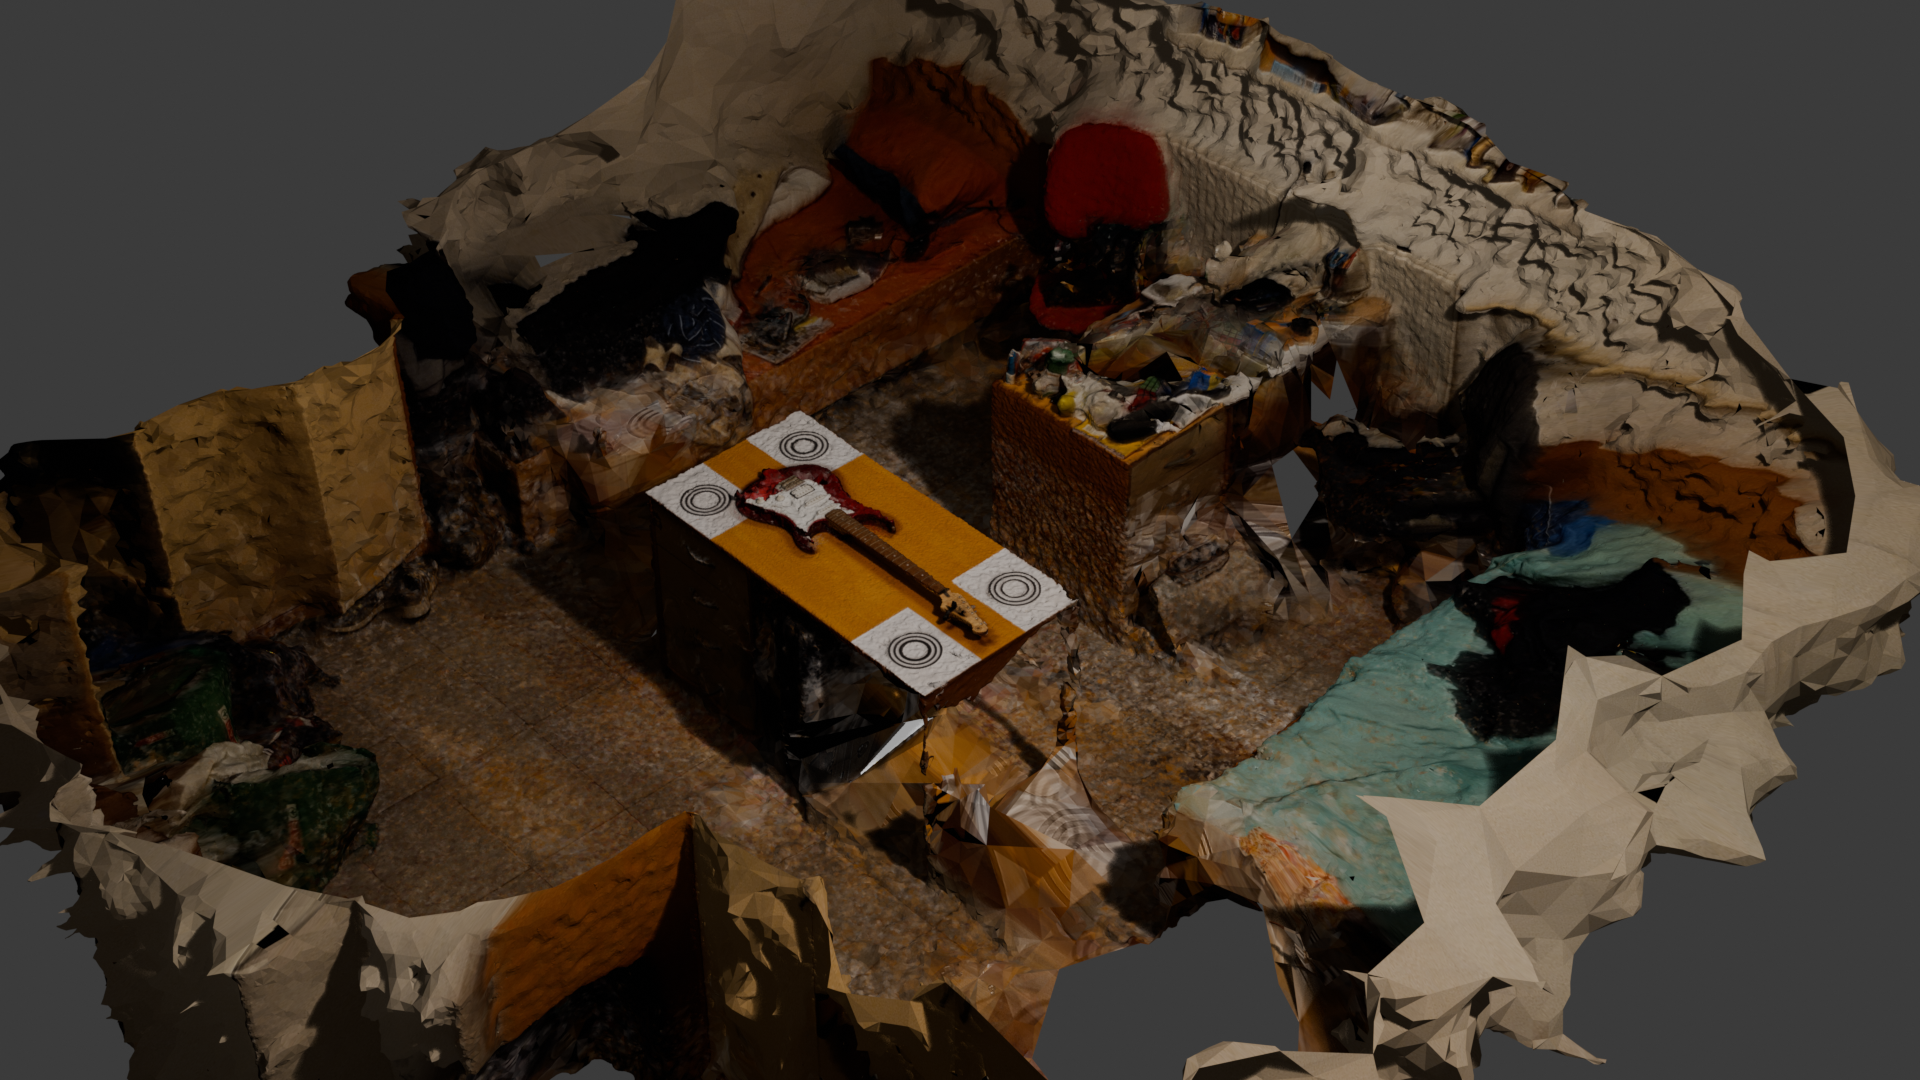
\includegraphics[width=.95\linewidth]{imgs/guitarsoba.png}
                \caption{Celoten rezultat iz Meshrooma}
            \end{subfigure}
            \begin{subfigure}{.5\textwidth}
                \centering
                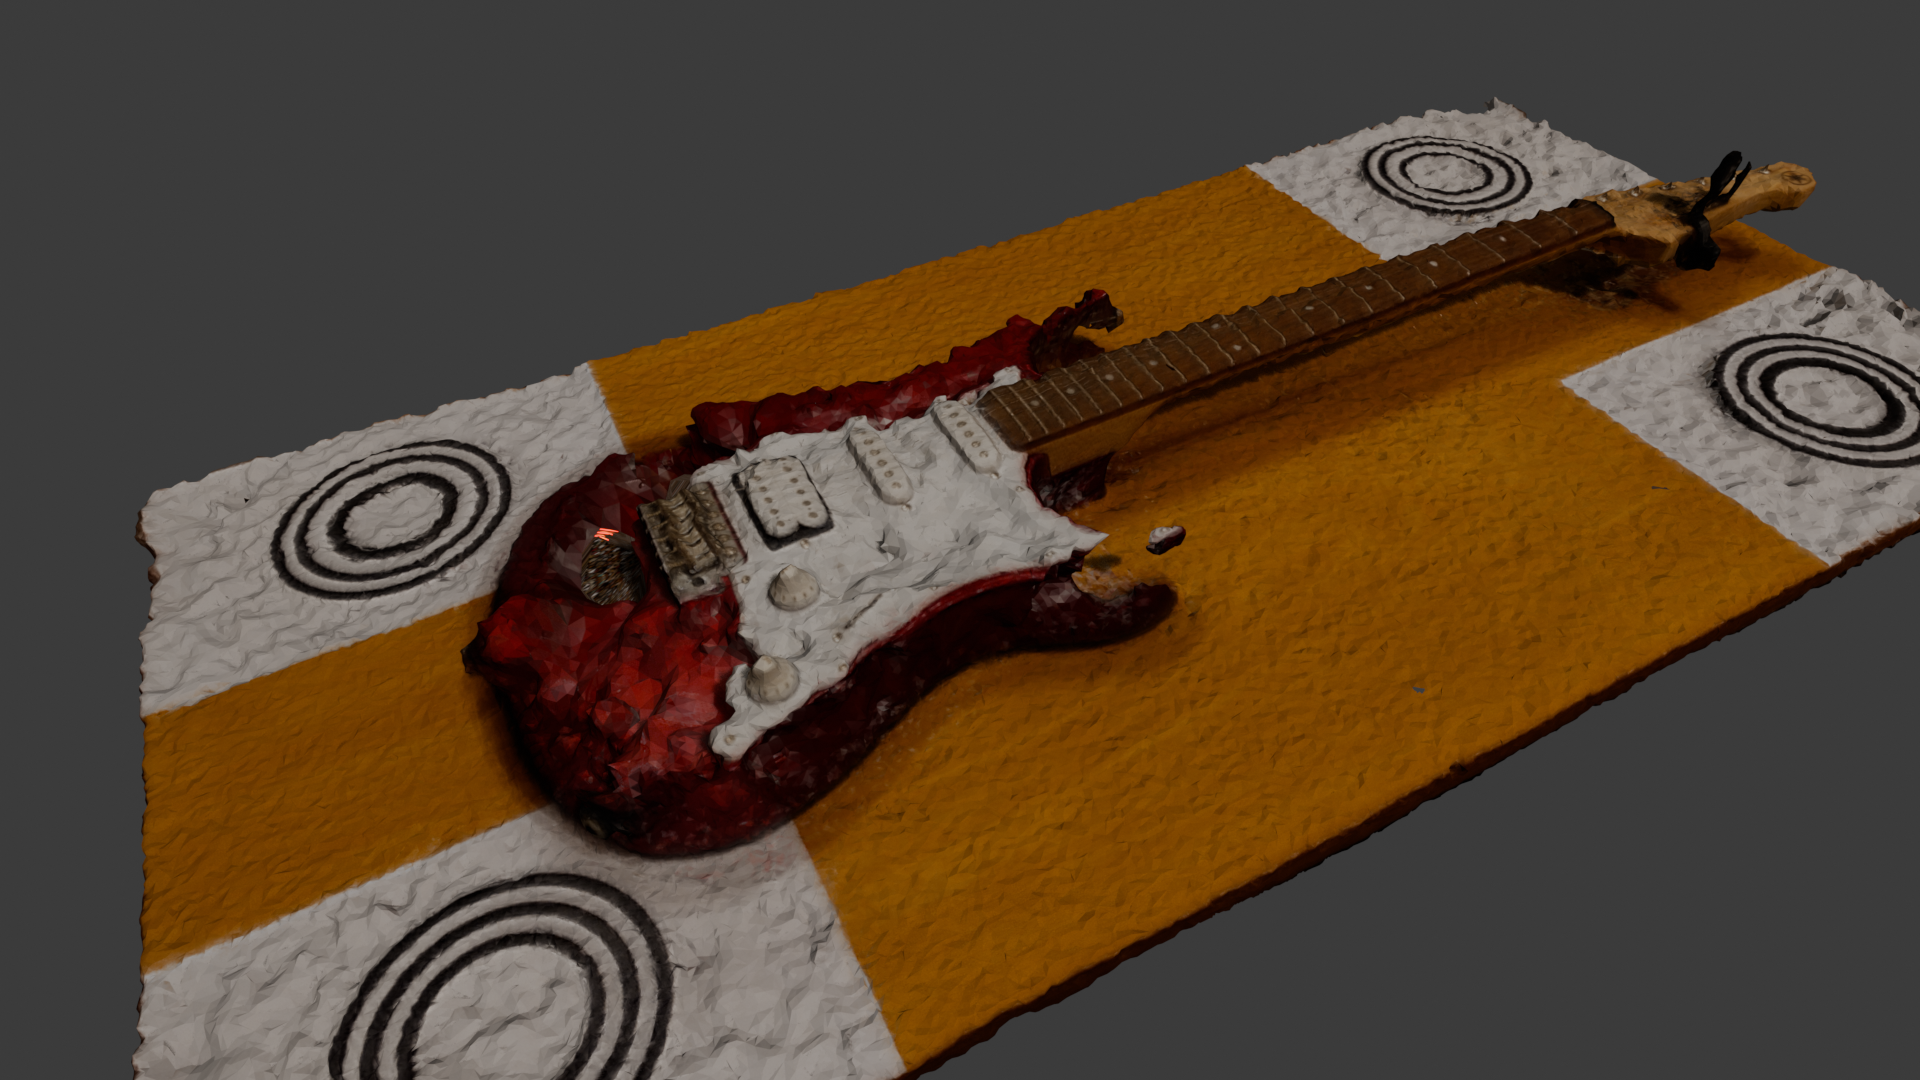
\includegraphics[width=.95\linewidth]{imgs/guitarcut.png}
                \caption{Izrezan rezultat}
            \end{subfigure}
            \caption{Rekonstrukcija kitare}
        \end{figure}
    
    \subsection{Veka}
        Ta model je bil narejen iz 34 slik moje modrice od blizu. Ideja je bila preizkusiti, koliko podrobnosti je mogoče ujeti na obrazu in modrici. Osvetlitev je bila namizna svetilka, usmerjena proti veki. Hitrost zaklopa je 1/20 s, ISO pa 150. Slike so bile posnete z ročnim telefonom. Rekonstrukcijo sem naredil z različnimi parametri, da jih je mogoče primerjati. Statistika o objektih je vidna v tabeli \ref{tab:objstat}. Vidimo lahko, da je za ta primer DSPSift veliko boljši od Akaze. Vidimo lahko tudi, da z višjimi nastavitvami dosežemo boljše rezultate, vendar je razlika med visoko in ultra zelo majhna. Iz spodnjih slik lahko opazimo, da ima Akaze veliko več ``valov" ykot DSPSift.  

        \begin{table}[h]
            \centering
            \begin{tabular}{|c|c|c|c|c|c|} \hline 
                 &  DSPSift Normal&  DSPSift High&  DSPSift Ultra&  DSPSift+Akaze& Akaze\\ \hline 
                 Vertices&  319630&  325135&  325175&  324528& 151640\\ \hline 
                 Edges&  952816&  968875&  969452&  967321& 451475\\ \hline 
                 Faces&  635128&  645823&  646201&  644784& 300898\\ \hline
            \end{tabular}
            \caption{Statistika objektov}
            \label{tab:objstat}
        \end{table}

        \begin{figure}[h]
            \begin{subfigure}{.5\textwidth}
                \centering
                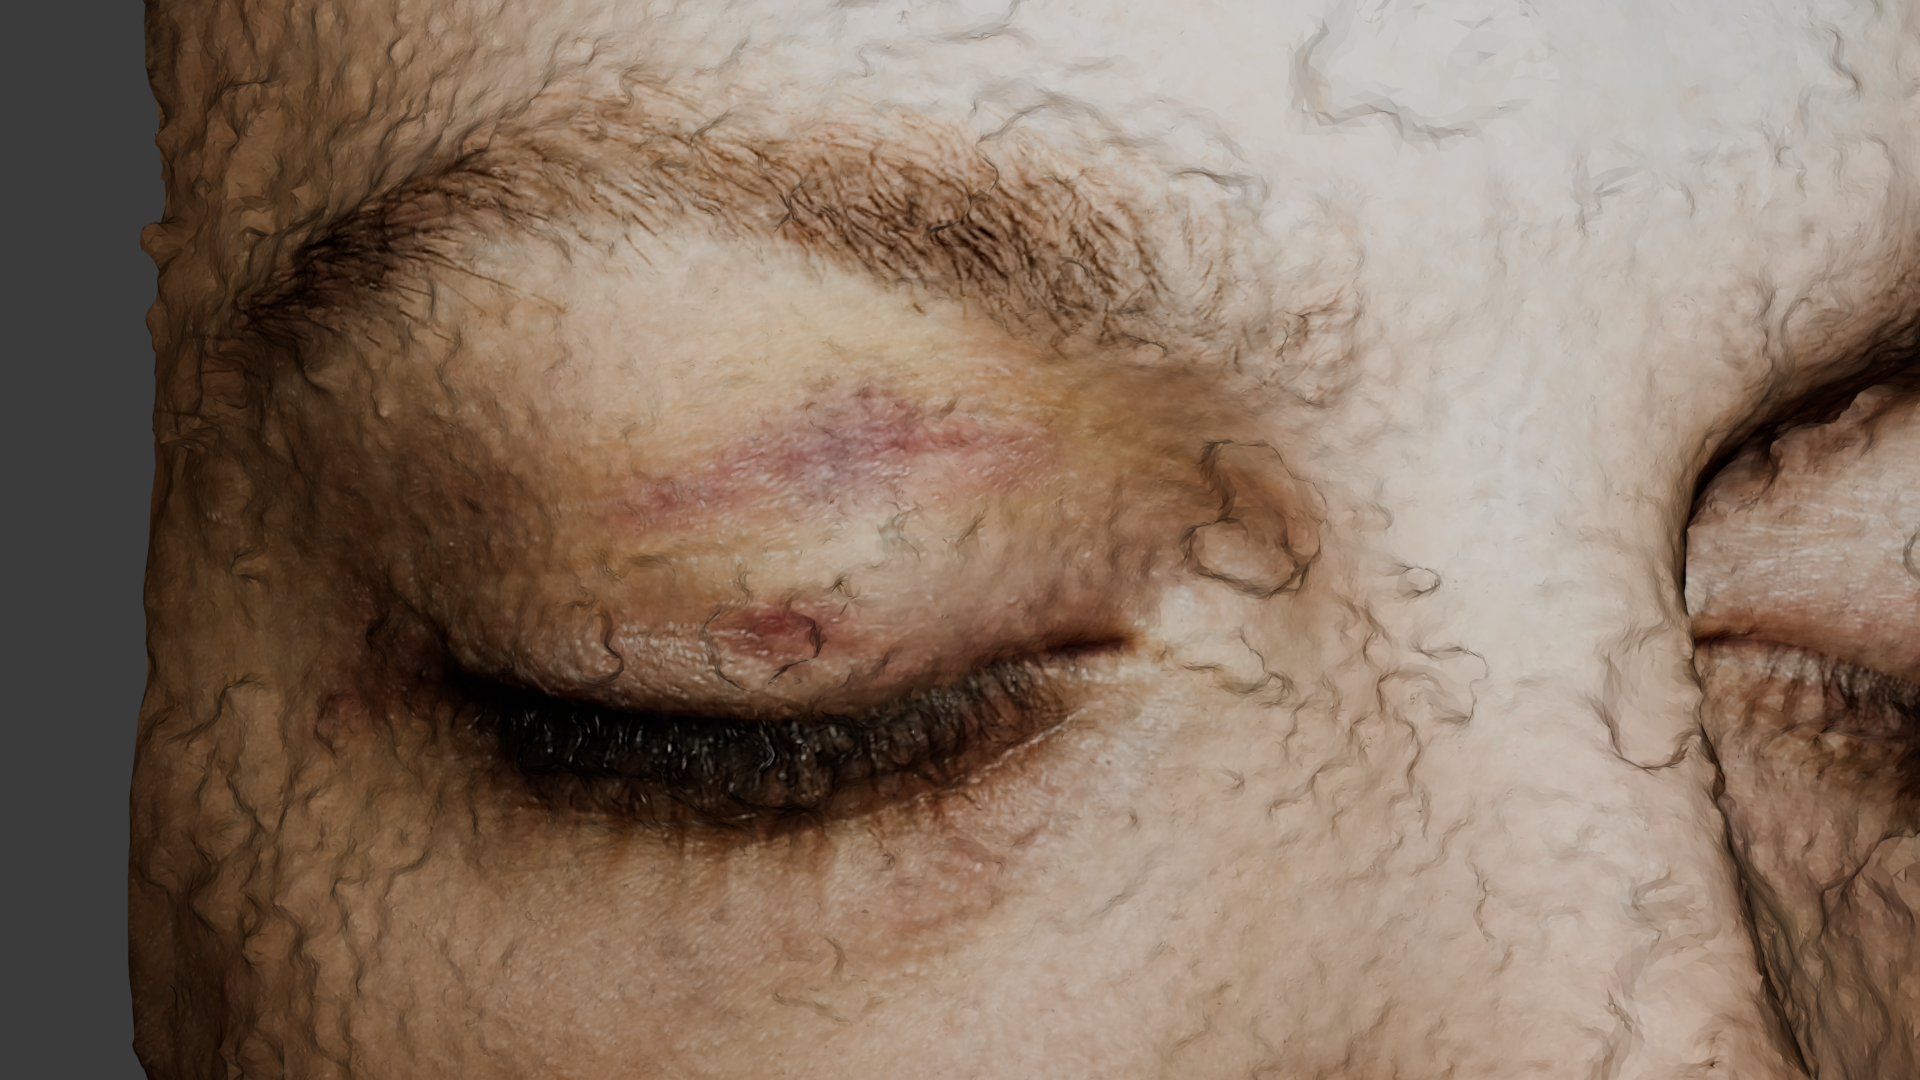
\includegraphics[width=.95\linewidth]{imgs/akaze.png}
                \caption{Akaze metoda}
            \end{subfigure}
            \begin{subfigure}{.5\textwidth}
                \centering
                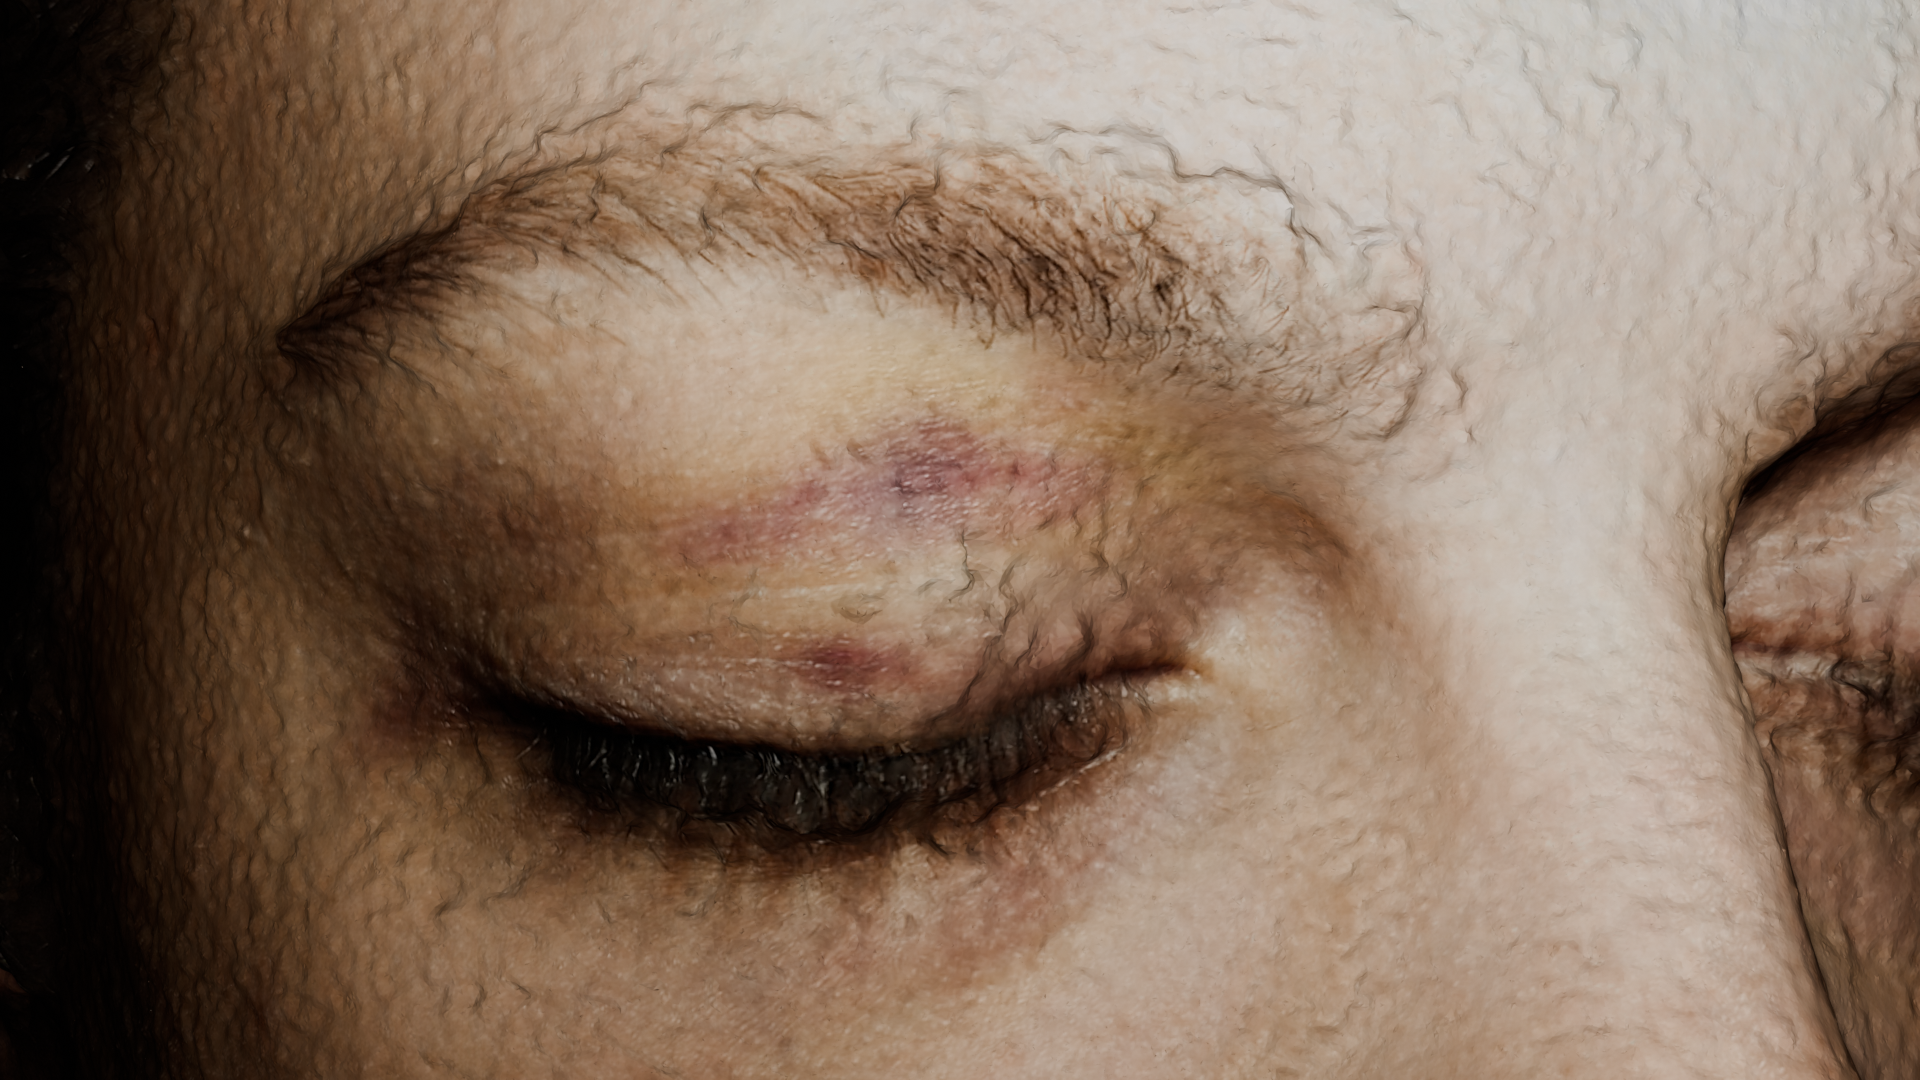
\includegraphics[width=.95\linewidth]{imgs/ultrarender.png}
                \caption{Ultra nastavitve}
            \end{subfigure}
            \caption{Rekonstrukcija vek}
        \end{figure}
    
    % \subsection{} %probaj parfem popravi ili arhitekt

    \subsection{Povzetek}
        Za dobro rekonstrukcijo moramo narediti dobre slike. Idealno bi bilo, da bi naš fotoaparat imel nižjo hitrost zaklopa in faktor ISO. Prav tako bi morali slikati v formatu JPEG in ne v formatu RAW. Osvetlitev je zelo pomembna. Moral bi biti neposredno na predmetu, ne sme ustvarjati senc. Zunanji objekt ne sme biti odseven, ker odboji svetlobnega vira povzročajo napake v rekonstruiranem modelu. Metoda DSPSift za ekstrakcijo funkcij je v preizkušenih primerih boljša od Akaze, morda pa bi bil Akaze primeren za težje površine. Nastavitve kakovosti in količine ekstrahiranih ``features" je treba spremeniti tudi glede na število slik in želeno raven podrobnosti.